\section{Evasión de colisiones}
\setlength{\columnseprule}{0pt}
\onecolumn
Los obstáculos son representados cinemáticamente mediante funciones anisotrópicas, las cuales ponderan la dirección relativa entre el agente y una posible colisión.
\setcounter{figure}{0}
\begin{figure}[H]
    \centering
    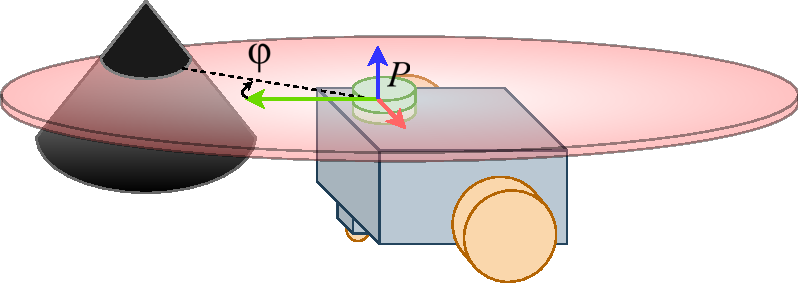
\includegraphics[width=0.5\linewidth]{Pics/angulo.pdf}
    \caption{Representación anisotrópica de un obstáculo}
    \label{fig:angulo}
\end{figure}